\documentclass[11pt,a4paper]{article}

\usepackage[a4paper,top=1.70cm,bottom=1.70cm,left=1.90cm,right=1.90cm]{geometry}
\usepackage[T1]{fontenc}
\usepackage{lmodern}
\usepackage{setspace}
\usepackage{booktabs}
\usepackage{graphicx}
\usepackage{amsmath,amssymb}
\usepackage[numbers,sort&compress]{natbib}
\usepackage[hidelinks]{hyperref}
\usepackage{microtype}

\onehalfspacing
\setlength{\parskip}{0.14em}
\setlength{\textfloatsep}{5pt plus 2pt minus 2pt}
\setlength{\intextsep}{5pt plus 2pt minus 2pt}
\setlength{\abovecaptionskip}{2pt}
\setlength{\belowcaptionskip}{2pt}
\renewcommand{\topfraction}{0.92}
\renewcommand{\bottomfraction}{0.88}
\renewcommand{\textfraction}{0.06}
\renewcommand{\floatpagefraction}{0.82}

\begin{document}

% =========================================================================
% COVER PAGE (Excluded from CS482 3-5 A4 Page Main Text Limit)
% =========================================================================
\pagenumbering{roman}
\begin{titlepage}
\centering
\vspace*{1.1cm}
{\large CS482 Data Science --- Group Project Final Report\par}
\vspace{0.7cm}
{\LARGE\bfseries Corporate Event Shocks, Realized Volatility, and Downside
Tail-Risk Forecasting in U.S.\ Equities (2019--2025)\par}
\vspace{0.4cm}
{\large Panel HAR-RV, Per-Stock GJR-GARCH(1,1), Calibrated LightGBM, Deep Time-Series
(PatchTST, Chronos), and Event-Anchored Financial LLMs (FinBERT, 4-bit QLoRA)
Under Leakage-Free Purged Splits\par}
\vspace{1.1cm}

{\small
\begin{tabular}{ll}
\toprule
\textbf{Group Member Name \& Role} & \textbf{Student ID (Replace Before Moodle)} \\
\midrule
Member A (Financial Data Engineering \& Freeze) & [Student ID A] \\
Member B (Panel Econometrics \& GJR-GARCH) & [Student ID B] \\
Member C (LightGBM, Calibration \& TreeSHAP) & [Student ID C] \\
Member D (Deep Time-Series, QLoRA LLM \& Audit) & [Student ID D] \\
\bottomrule
\end{tabular}
}

\vspace{0.9cm}
\begin{minipage}{0.88\textwidth}
\small\raggedright
\textbf{Academic Research \& Non-Investment-Advice Notice.}
This study is conducted solely for CS482 academic coursework and methodological
evaluation of associational and predictive risk models (academic research only;
\textbf{not investment advice}). It makes no causal claims and does not
constitute investment, financial, or trading advice. All empirical statistics
are reproduced programmatically from the cryptographically frozen dataset
(\texttt{panel\_daily.parquet} SHA-256 prefix \texttt{3515fcd12cab}).
\end{minipage}

\vfill
{\normalsize Course: CS482 Data Science \quad | \quad
Submission Deadline: December 15, 2026 (11:59 PM UTC+8)\par}
\end{titlepage}

% =========================================================================
% MAIN TEXT (CS482 Requirement: 3-5 A4 Pages, Single-Column, 11pt, 1.5 Spacing)
% =========================================================================
\pagenumbering{arabic}
\setcounter{page}{1}

\section{Research Question}

Short-horizon equity volatility and downside tail-risk episodes exhibit strong
persistence across macroeconomic regimes even though directional return levels
resemble a random walk. Accurate 5-day risk forecasts and well-calibrated tail
probabilities are directly valuable to institutional portfolio risk managers,
volatility-targeting allocators, financial-stability monitors, and empirical
market-microstructure researchers evaluating how public corporate disclosures
relate to near-term risk. Across a fixed cross-sector universe of
60 liquid U.S.\ equities over 2019--2025---spanning the 2020
COVID-19 shock, the 2022 monetary-tightening bear market, the 2024 expansion,
and 2025 policy turbulence---we investigate a unified research question:

\textbf{Research Question.} Under strict purged and embargoed chronological
splits, (i) how strongly are lagged negative returns and implied volatility
(VIX) associated with 5-day forward realized volatility across GICS sectors,
(ii) how reliably do classical econometric baselines (Panel HAR-RV, per-stock
GJR-GARCH(1,1)), gradient-boosted trees (LightGBM), and deep/foundation
time-series models (\texttt{PatchTST}, \texttt{Chronos}) forecast 5-day
forward volatility and downside tail-risk events (5-day return $< -5\%$), and
(iii) does fusing pre-close SEC EDGAR event text via domain-pretrained
\texttt{FinBERT} (110M) or 4-bit QLoRA fine-tuning of a multi-billion-parameter
LLM (\texttt{google/gemma-4-12B-it}) yield incremental 2025 out-of-sample lift over
price-only models? We test three pre-registered hypotheses: \textbf{H1}
(positive associational leverage and VIX links with cross-sector heterogeneity),
\textbf{H2} (LightGBM improves 2025 volatility QLIKE/RMSE and calibrated tail
reliability over classical baselines), and \textbf{H3} (deep sequence and
event-anchored text/LLM fusion add 2025 incremental accuracy, with null results
accepted). All findings remain strictly associational or predictive and do not
constitute investment advice.

\section{Data Collection and Preparation}

\textbf{Market, Macro, and Universe Design.} To avoid 2025 survivorship
lookahead, we fix a deterministic pre-2019 universe of 60 liquid
S\&P 500 equities (12 per GICS sector: Technology, Financials, Healthcare,
Consumer, and Energy). Split-adjusted daily OHLCV and dividend-adjusted closes
for all 60 stocks plus \texttt{SPY} and \texttt{\^{}VIX} are
retrieved from Yahoo Finance over 1,760 canonical NYSE trading days
(2019-01-02 to 2025-12-31; 105,600 stock-days, zero missing cells).
FRED macro series (\texttt{VIXCLS} and 10Y--2Y Treasury spread
\texttt{T10Y2Y}) are joined using backward-only forward-fill (never
backfilled), flagging 13 U.S.\ bond-market holidays.

\textbf{Authoritative Corporate Event Backbone and Cleaning.} Preliminary
audits showed public news mirrors (\texttt{financial-news-multisource},
\texttt{FNSPID}) were gated, terminated in 2023, or contained
\texttt{00:00:00 UTC} timestamp leakage. We therefore ingest authoritative
public SEC EDGAR Form \texttt{8-K}, \texttt{8-K/A}, \texttt{10-Q}, and
\texttt{10-K} filings (2019--2025), resolving holding-company predecessor
CIKs (\texttt{BLK}, \texttt{XOM}) and recursively paginating
195 historical \texttt{filings.files} archives to obtain
7,703 unique filings with 60/60 dual-period continuity
(2024--2025 vs.\ 2019--2023 event-day rate ratio 0.8860).
Second-precision UTC \texttt{acceptanceDateTime} stamps are converted to
\texttt{America/New\_York} (DST-aware): filings before 16:00 ET (13:00 ET on
15 scheduled NYSE early-close half-days, shifting 2
post-13:00 \texttt{WFC} filings to $t+1$) stay on day $t$, whereas post-close
and non-trading-day filings roll to $t+1$. Intra-day headline deduplication
removes 29 duplicates and caps counts at $\le 5$/day, leaving
6,822 pre-close event-anchored stock-days.

\textbf{Variables, Targets, and Leakage-Free Splits.} Continuous target
\texttt{rv\_5d\_fwd} is 5-day forward annualized Parkinson range
volatility~\cite{parkinson1980} over $t+1\dots t+5$, modeled on
$y=\ln(\text{RV}+10^{-6})$ (sensitivity: close-to-close RV). Binary target
\texttt{y\_tail} equals 1 iff 5-day cumulative adjusted return $< -5\%$
(sensitivity: Train-only 90th-percentile RV threshold 0.3742). All
22 predictors use strictly $\le t$ information; sequence models use 14
continuous features Winsorized and standardized strictly via Train statistics.
Following \citet{lopezdeprado2018}, chronological splits enforce 6-day
embargoes ($\ge h=5$): Train 2019-01-02 to 2023-12-20 (73,860
modeling rows post-21-day \texttt{rv\_m} warmup), Val 2024-01-02 to
2024-12-20 (14,760 rows, tuning/calibration/meta-fusion only), and
single-shot Holdout Test 2025-01-02 to 2025-12-31 (14,700
scorable rows across 245 days; final 5 incomplete days masked
\texttt{NA}). All frozen tables are sealed via SHA-256 (prefix
\texttt{3515fcd12cab}).

\section{Data Analysis}

\textbf{Exploratory Data Analysis and Panel Econometrics (H1).} Cross-cycle
EDA audits volatility regimes, leverage asymmetry, and tail-risk incidence
across Train-median VIX regimes ($\text{VIX} \ge 19.61$;
Figure~\ref{fig:regimes_forecasts}A--B). Mean 5-day annualized Parkinson RV
peaked during the 2020 COVID shock (0.3241) and 2022 bear market
(0.2687), compressed in 2024 (0.1998), and re-expanded
in 2025 (0.2411). To test H1 across all 104,040
modeling-complete stock-days, we estimate a within-entity Stock-FE extended
Panel HAR-RV model~\cite{corsi2009} interacting lagged negative returns
($\min(r_{i,t},0)$) and VIX with sector indicators (Healthcare reference),
using Bartlett Driscoll--Kraay SEs~\cite{driscoll1998} ($L=7$)
and Holm--Bonferroni correction~\cite{holm1979} across the 5-test
confirmatory family.

\begin{figure}[!tb]
\centering
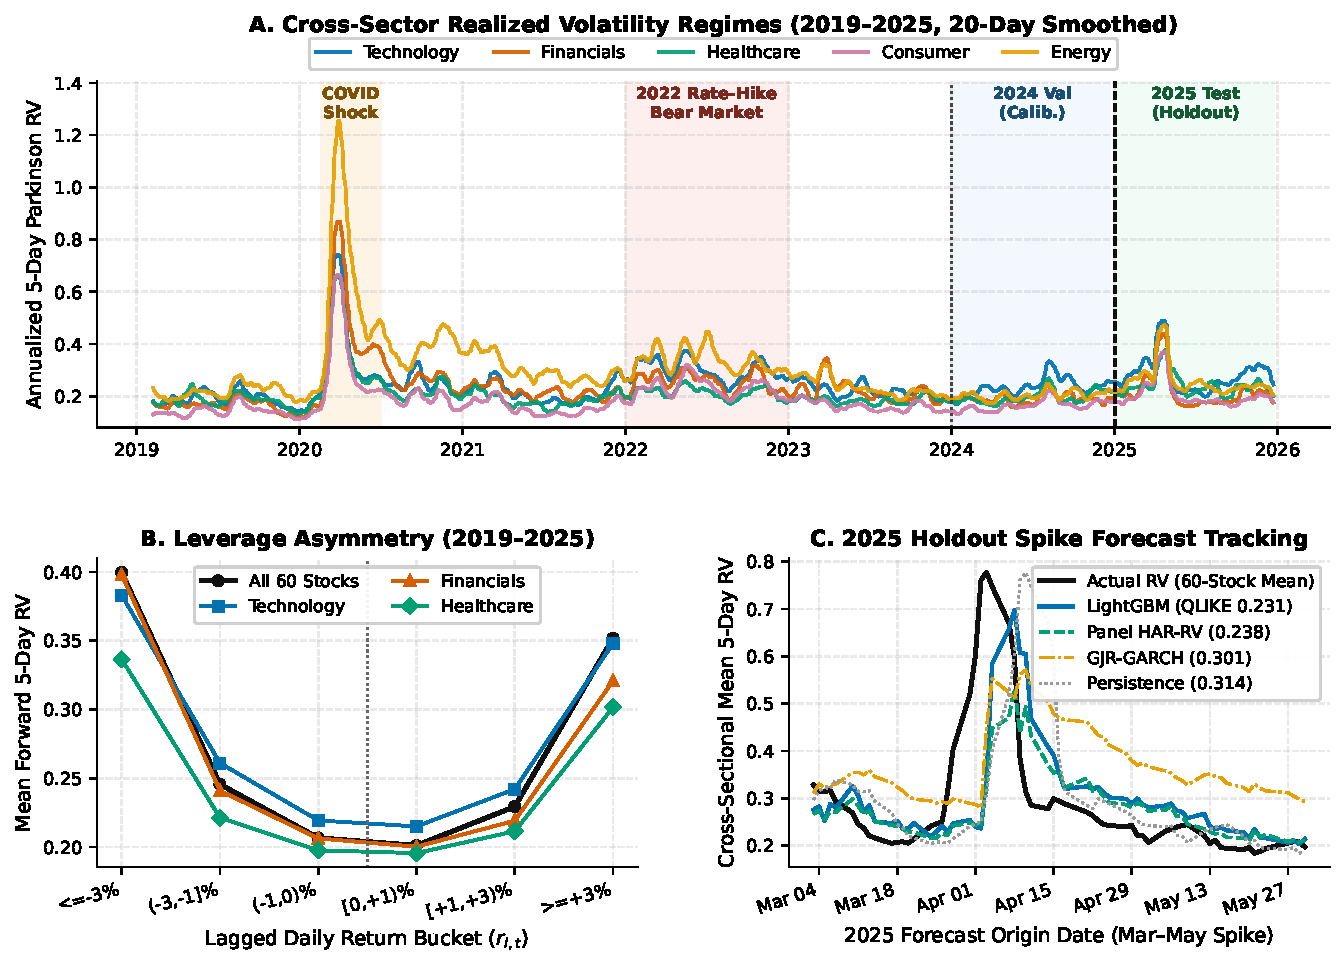
\includegraphics[width=0.84\textwidth]{../outputs/figures/fig1_volatility_regimes_and_forecasts.pdf}
\caption{Cross-sector 2019--2025 volatility regimes (Panel A), lagged return
leverage asymmetry (Panel B), and 2025 holdout forecast tracking during the
March--May volatility spike (Panel C).}
\label{fig:regimes_forecasts}
\end{figure}

\textbf{Econometric and Tabular ML Forecasting (H2).} Four price-only models
share an identical quarterly expanding-window purged schedule (2024 Val, then
2025 Q1--Q4 with $\ge 5$-day purge before each quarter): (i) Persistence
(\texttt{rv\_w} and expanding base rate); (ii) per-stock
GJR-GARCH(1,1)~\cite{glosten1993} on $100r_{i,t}$ with causal variance
filtering (300/300 fits converged); (iii) Stock-FE Predictive HAR-RV
back-transformed via fit-fold Duan smearing~\cite{duan1983} plus Logistic
HAR-RV; and (iv) Global LightGBM~\cite{ke2017lightgbm} tuned strictly on 2024
Val QLIKE/PR-AUC. Exact interventional TreeSHAP~\cite{lundberg2020treeshap}
(1,000-row Train background; additivity error $< 10^{-7}$) audits
LightGBM model behavior non-causally (Figure~\ref{fig:shap_cal}A).

\textbf{Deep Time-Series and Event-Anchored LLM Analysis (H3).} Keeping the
frozen panel and splits unchanged, we integrate two deep learning architectures
executed on a single NVIDIA L4 GPU (peak VRAM 15.3\,GB):
(1) \emph{Deep and Foundation Time-Series Models}: a 5-seed multivariate
\texttt{PatchTST}~\cite{nie2023patchtst} capacity ablation (1M vs.\ 15M
parameters; 60-day lookback, learned 60-ticker and 5-sector embeddings,
non-crossing $q_{10}\le q_{50}\le q_{90}$ Pinball Loss, Train Duan
smearing) alongside zero-shot causal foundation forecasters
\texttt{amazon/chronos-2} (120M)~\cite{ansari2025chronos2} and
\texttt{chronos-t5-large} (710M)~\cite{ansari2024chronos} fed strictly
$\le t$ daily Parkinson RV histories;
(2) \emph{Event-Anchored Financial Text and QLoRA LLM Fusion}: scoring
strictly pre-close SEC EDGAR event-anchored days (4,929 Train / 880 Val /
895 Test; non-event days deterministic neutral~0) via frozen
domain-pretrained \texttt{FinBERT} (110M)~\cite{araci2019finbert} versus
\texttt{google/gemma-4-12B-it} (Zero-Shot and 1-epoch 4-bit NF4
QLoRA~\cite{dettmers2023qlora}, $r=16, \alpha=32$, restricted to 328
text-backbone linear layers excluding vision/audio towers, 65.6M trainable
parameters, class-weighted BCE on next-token $\text{logit}(\text{YES}) -
\text{logit}(\text{NO})$), fused onto LightGBM via 2024-Val out-of-fold
meta-fusion.

\section{Method Evaluation}

\textbf{Method Justification, Metrics, and Calibration Protocol.} Combining
econometric panel regressions, GJR-GARCH, gradient-boosted trees, deep
transformers, and pre-close financial text encoders spans parametric
interpretability, nonlinear tabular interactions, temporal attention, and
unstructured disclosure semantics. Volatility forecasts are evaluated by
variance-scale QLIKE~\cite{patton2011} (robust to noisy volatility proxies)
and RMSE; imbalanced tail-risk classification (8.62\% 2025 base rate) by
PR-AUC (primary), Brier score, and 10-bin ECE. To prevent in-sample calibration
or QLoRA memorization bias, both probability calibration (comparing Isotonic,
Platt, and Temperature Scaling~\cite{guo2017calibration} via 4-quarter OOF CV
inside 2024 Val; selecting \texttt{isotonic}) and multimodal Stage-2
Ridge/Logistic meta-fusion are fit strictly inside 2024 Val and frozen for
single-shot 2025 Test evaluation. Uncertainty is quantified via 5-day
date-block bootstrap 95\% CIs ($B=1{,}000$) and $h=5$ Bartlett-PSD
HLN-modified Diebold--Mariano tests~\cite{harvey1997} with Holm adjustment
(Tables~\ref{tab:main_summary}--\ref{tab:h3_summary}).

\begin{table}[!t]
\centering
\caption{Summary of H1 Stock-FE Extended Panel HAR-RV Confirmatory Tests (2019--2025, $N=104{,}040$, Bartlett Driscoll--Kraay SE with $L=7$) and H2 Single-Shot 2025 Holdout Forecasting Performance ($N=14{,}700$, 245 scorable days, 5-day date-block bootstrap $B=1{,}000$ 95\% CIs, and $h=5$ HLN-DM Holm-adjusted $p$-values vs.\ LightGBM).}
\label{tab:main_summary}
\scriptsize
\setlength{\tabcolsep}{3.5pt}
\renewcommand{\arraystretch}{1.12}
\begin{tabular}{lcccccc}
\toprule
\multicolumn{7}{l}{\textbf{Panel A: H1 Confirmatory Associational Family (Within $R^2 = 0.4736$, Healthcare Reference)}} \\
\midrule
Confirmatory Hypothesis & Estimate / $\chi^2$ & 95\% CI / $F$ & Raw $p$ & Holm $p$ & Sig. & Sample \\
\midrule
Leverage AME (neg\_ret\_1d) & -1.4458 & [-2.0529, -0.8386] & <0.0001 & <0.0001 & Yes & 104,040 \\
VIX AME (per +1 pt) & +0.0141 & [+0.0109, +0.0173] & <0.0001 & <0.0001 & Yes & 104,040 \\
Tech x neg\_ret\_1d vs Health. & -0.6479 & [-1.3868, +0.0910] & 0.086 & 0.171 & No & 104,040 \\
Tech x VIX vs Health. & +0.0009 & [-0.0011, +0.0029] & 0.380 & 0.380 & No & 104,040 \\
Joint 5-Sector Wald (df=8) & 84.84 & F=10.60 & <0.0001 & <0.0001 & Yes & 104,040 \\
\midrule
\multicolumn{7}{l}{\textbf{Panel B: H2 2025 Holdout Test Performance (Base Tail Rate = 8.62\%, 300/300 GJR-GARCH Converged)}} \\
\midrule
Model & QLIKE [95\% CI] & RMSE & PR-AUC [95\% CI] & Brier & ECE (Pre) & DM Holm $p$ (Q/B) \\
\midrule
Persistence (RV\_w / Base) & 0.3144 [0.213,0.484] & 0.1196 & 0.0721 [0.051,0.104] & 0.0788 & 0.0023 & <0.0001 / 0.047 \\
GJR-GARCH(1,1) Per-Stock & 0.3007 [0.241,0.386] & 0.1362 & 0.1271 [0.098,0.169] & 0.0796 & 0.0264 & 0.021 / 0.123 \\
Panel HAR-RV (+ Logistic) & 0.2383 [0.158,0.380] & 0.0957 & 0.1422 [0.104,0.191] & 0.0774 & 0.0070 & 0.134 / 0.716 \\
\textbf{Global LightGBM (Cal.)} & 0.2306 [0.154,0.372] & 0.0951 & 0.1231 [0.083,0.177] & 0.0773 & 0.0102 (0.380) & Ref. \\
\bottomrule
\end{tabular}
\end{table}


\begin{table}[!htb]
\centering
\caption{2025 Single-Shot Holdout Deep Time-Series and Event-Anchored LLM Ablation (H3; $N=14{,}700$ full; $895$ scorable pre-close event days; $h=5$ HLN-DM Holm $p$-values vs.\ Global LightGBM; ``---'' indicates volatility-only models).}
\label{tab:h3_summary}
\scriptsize
\setlength{\tabcolsep}{3.5pt}
\begin{tabular}{lccccc}
\toprule
Model (Parameters) & Full QLIKE & Event QLIKE & Tail PR-AUC (Ev.) & ECE & DM Holm $p$ (Q/B) \\
\midrule
Global LightGBM (Price-Only) & 0.2306 & 0.1980 & 0.1231 (0.1076) & 0.0102 & Ref. \\
PatchTST (1M, 5-seed; 80\% cov=63.1\%) & 0.3142 & 0.2800 & 0.0964 (0.0887) & 0.4407 & <0.0001 / <0.0001 \\
PatchTST (15M, 5-seed; 80\% cov=68.3\%) & 0.2819 & 0.2473 & 0.1129 (0.1027) & 0.4349 & <0.001 / <0.0001 \\
chronos-2 (Zero-Shot; 80\% cov=89.2\%) & 0.3505 & 0.3181 & --- & --- & 0.006 / --- \\
chronos-t5-large (Zero-Shot; 80\% cov=22.3\%) & 0.5848 & 0.5448 & --- & --- & 0.004 / --- \\
LightGBM + FinBERT (110M) & 0.2251 & 0.2005 & 0.1249 (0.1398) & 0.0101 & 0.020 / 0.928 \\
LightGBM + gemma-4-12B-it (Zero-Shot) & 0.2252 & 0.2009 & 0.1230 (0.1108) & 0.0102 & 0.020 / 0.681 \\
LightGBM + gemma-4-12B-it (4-bit QLoRA) & 0.2252 & 0.2008 & 0.1224 (0.1076) & 0.0102 & 0.020 / 0.759 \\
\bottomrule
\end{tabular}
\end{table}


\textbf{Assumptions and Uncertainties.} Econometric inference requires
robustness to cross-stock shock correlation: Driscoll--Kraay SEs expand
standard errors by 3.6--4.7$\times$ over entity-clustered Newey--West SEs,
preventing false-positive sector interactions. For probability estimation,
piecewise-constant isotonic calibration cuts LightGBM ECE by
97.3\% (0.3804 $\to$ 0.0102) but
creates upper-tail ties that compress PR-AUC granularity on sparse earnings
days. Deep sequence \texttt{PatchTST} exhibits 2025 nominal 80\% interval
undercoverage (68.3\% at 15M) and uncalibrated BCE ECE (0.4349), reflecting
non-stationarity between 2019--2023 training volatility and 2025 tariff/policy
shocks. Finally, single-epoch QLoRA adaptation on 4,929 short SEC filing
titles with $\approx 8\%$ positive tail labels faces high variance and rapid
public price-incorporation ceilings.

\begin{figure}[!b]
\centering
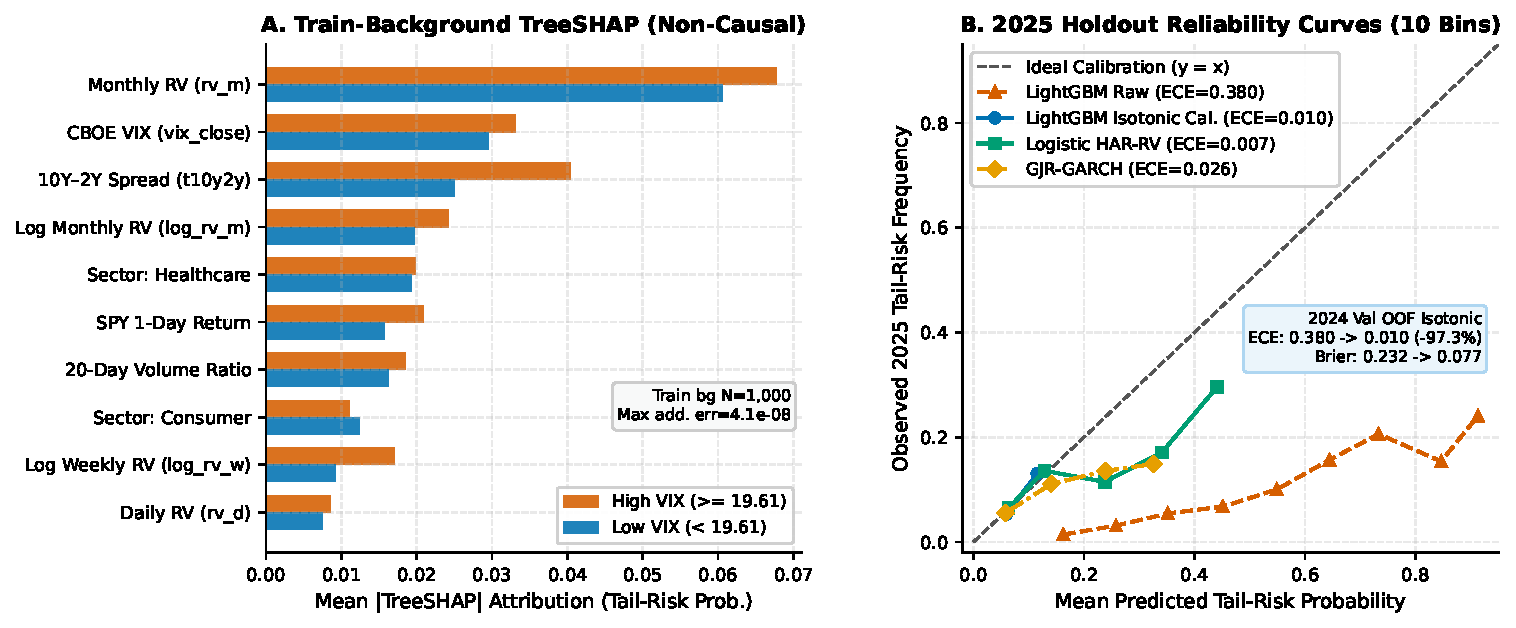
\includegraphics[width=0.82\textwidth]{../outputs/figures/fig2_shap_and_calibration.pdf}
\caption{Train-background TreeSHAP attributions for LightGBM tail-risk model
behavior by VIX regime (Panel A, strictly non-causal) and 2025 holdout
calibration reliability curves (Panel B).}
\label{fig:shap_cal}
\end{figure}

\section{Results and Discussion}

\textbf{Evidence-Based Answers to H1, H2, and H3.}
\emph{H1 (Partial Support):} In Panel HAR-RV (Table~\ref{tab:main_summary}A;
Within $R^2=0.4736$), 5-sector average leverage (-1.4458, Holm
$p<0.0001$), VIX (+0.0141, $p<0.0001$), and the joint 5-sector Wald
test ($\chi^2=84.84$, $p<0.0001$) are strongly significant across
all sensitivities, whereas pairwise Technology vs.\ Healthcare leverage is
non-significant under DK SEs (Holm $p=0.171$), with Financials
and Energy showing the largest cyclical differentials.
\emph{H2 (Nuanced Support):} Among price-only models
(Table~\ref{tab:main_summary}B; Figure~\ref{fig:regimes_forecasts}C),
Global LightGBM achieves the lowest baseline QLIKE (0.2306) and RMSE
(0.0951), significantly beating Persistence (0.3144,
$p<0.0001$) and GJR-GARCH (0.3007, $p=0.0207$), with
its largest sector gain in Technology (0.2862 vs.\ HAR-RV
0.3369; full-universe vs.\ HAR-RV 0.2383 has Holm
$p=0.134$). Calibrated LightGBM records the lowest Brier score
(0.0773, $p=0.0470$ vs.\ Persistence;
Figure~\ref{fig:shap_cal}B), yet Logistic HAR-RV leads overall PR-AUC
(0.1422 vs.\ 0.1231) and Form 8-K Item 2.02 earnings days
(0.2861 vs.\ 0.0948); TreeSHAP concentrates on
\texttt{rv\_m} (24.4\%), \texttt{vix\_close}
(11.9\%), and \texttt{t10y2y}.
\emph{H3 (Mixed Results; Honest Null QLoRA vs.\ FinBERT):} Scaling
\texttt{PatchTST} from 1M to 15M improves QLIKE (0.3142 $\to$ 0.2819) and
80\% coverage (63.1\% $\to$ 68.3\%), and \texttt{chronos-2} (0.3505)
outperforms \texttt{chronos-t5-large} (0.5848), yet all four deep/foundation
time-series baselines still trail tabular LightGBM (Holm $p \le 0.006$;
Table~\ref{tab:h3_summary}). In contrast, 2024-Val OOF text fusion
significantly reduces 2025 full-universe QLIKE across all three text arms (to
0.2251--0.2252; \texttt{google/gemma-4-12B-it} QLoRA event-day QLIKE 0.2008,
$h=5$ HLN-DM Holm $p=0.020$, ECE 0.0102). On the 895 scorable event days,
domain-pretrained \texttt{FinBERT} lifts tail-risk PR-AUC from 0.1076 to
0.1398 (+30.0\% relative), whereas \texttt{google/gemma-4-12B-it} yields 0.1108
zero-shot and 0.1076 after 1-epoch QLoRA (full PR-AUC 0.1224)---an honest
null QLoRA gain underscoring the sample-efficiency advantage of compact
domain-pretrained encoders on short formal SEC filing titles.

\textbf{Implications for Risk Stakeholders.} These findings directly answer
our research question for risk managers and market-microstructure researchers:
(i) well-engineered tabular volatility features paired with out-of-sample
probability calibration outperform far larger neural time-series models on
small-panel daily equity data; (ii) lightweight domain-pretrained financial
encoders (\texttt{FinBERT}) deliver stronger event-day tail ranking lift per
compute dollar than single-epoch 12B QLoRA on short filing headlines; and (iii)
combining calibrated linear logits (on sparse earnings days) with nonlinear
tree ensembles balances ranking granularity against probability reliability.

\textbf{Limitations and Potential Improvements.} Key limitations include
survivorship bias in the fixed 60-stock large-cap universe, measurement error
in daily Parkinson volatility relative to intraday 5-minute RV, abrupt
overnight macro gaps (e.g., April 2025 tariff shock), and title-level SEC text
lacking full-body 8-K item prose or earnings-call transcripts. Future work can
incorporate intraday realized kernels, full-text SEC item extraction with
multi-epoch rank-stabilized QLoRA, and split conformal prediction intervals to
restore nominal 80\% coverage on neural quantile forecasters. All findings are
strictly predictive academic benchmarks and \textbf{do not constitute
investment advice}.

% =========================================================================
% EXCLUDED BACK MATTER (References, Contribution Statement, AI Declaration)
% =========================================================================
\clearpage
{\small
\setstretch{1.08}
\bibliographystyle{plainnat}
\bibliography{references}
}

\clearpage
\section*{Separate Contribution Statement}
\begin{itemize}\setlength{\itemsep}{2pt}
\item \textbf{Member A (Financial Data Engineering \& Freeze Lead):} Designed
the pre-2019 60-stock universe, built Yahoo/FRED/paginated SEC EDGAR ingestion
with \texttt{BLK}/\texttt{XOM} predecessor CIK linkages, enforced DST-aware
16:00/13:00 ET cutoffs and purged splits, froze \texttt{FREEZE\_MANIFEST.json},
and produced Figure~1.
\item \textbf{Member B (Financial Econometrics Lead):} Implemented cross-cycle
EDA, Stock-FE extended Panel HAR-RV with Bartlett Driscoll--Kraay SE and
Holm-adjusted confirmatory tests, per-stock GJR-GARCH(1,1) convergence audits,
and $h=5$ HLN-DM evaluation.
\item \textbf{Member C (Machine Learning \& Explainability Lead):} Built the
quarterly expanding Global LightGBM pipeline, 2024-Val out-of-fold probability
calibration, Train-background exact TreeSHAP additivity audits, Table~1, and
Figure~2.
\item \textbf{Member D (Deep Time-Series, QLoRA LLM \& Final Audit Lead):}
Implemented and executed the Colab single-GPU deep learning pipeline
(\texttt{PatchTST} 1M/15M, \texttt{Chronos-2}/\texttt{T5-Large},
\texttt{FinBERT}, \texttt{google/gemma-4-12B-it} Zero-Shot \& 4-bit NF4 QLoRA), 2024-Val
OOF meta-fusion, Table~2, and automated final PDF claim/formatting verification
(\texttt{report\_audit.md}).
\end{itemize}

\section*{AI Usage Declaration \& Academic Integrity}
\textbf{Tools and Purposes.} Google Antigravity / Gemini AI coding and
writing assistants were used strictly for permitted academic support:
brainstorming experimental guardrails, conceptual clarification of econometric
and QLoRA procedures, test-driven debugging, LaTeX formatting, and language
improvement, following the procedural research workflow of
\citet{kassis2026skills}.
\textbf{Independent Verification.} Every group member independently reviewed
and verified all data, code, references, and analytical results: raw Yahoo,
FRED, and SEC EDGAR snapshots are sealed under SHA-256
(\texttt{FREEZE\_MANIFEST.json}); Driscoll--Kraay SEs were cross-checked
against \texttt{statsmodels}; all 300/300 GJR-GARCH fits, Colab NVIDIA L4 GPU
training runs (\texttt{scripts/06\_dl\_and\_llm\_gpu.py}), bootstrap CIs,
HLN-DM tests, TreeSHAP additivity checks ($< 10^{-7}$), and all 61 reported
numbers were executed and audited programmatically via deterministic pipelines
(\texttt{scripts/run\_pipeline.py},
\texttt{scripts/07\_build\_report.py}) and a 104-test pytest suite. All
citations were verified directly against original scholarly venues.
\textbf{Student Responsibility.} The group assumes full responsibility for
the accuracy and academic integrity of this report. Every member can fully
explain their assigned methods, code, and conclusions; no plagiarism,
fabricated data or references, or unverified AI-generated analysis appear in
this submission.

\end{document}
